% !TeX program = xelatex
\documentclass[a4paper,10pt]{article}

% ============================================================================
% កញ្ចប់បណ្ណាល័យ (Packages) – តាមលំនាំស្តង់ដារអនុវិទ្យាល័យព្រះក្រសាំង (ls_plan.tex)
% ============================================================================
\usepackage[a4paper, left=0.95cm, right=0.95cm, top=0.85cm, bottom=0.92cm, footskip=0.52cm]{geometry}
\usepackage{amsmath}
\usepackage{unicode-math}
\usepackage{fontspec}
\usepackage{array, longtable, multirow, colortbl}
\usepackage[table]{xcolor}
\usepackage{enumitem}
\usepackage{pifont}
\usepackage{fancyhdr}
\usepackage{tikz}
\usetikzlibrary{calc, arrows.meta, angles, quotes, decorations.markings, babel}

% LaTeX 2025 + longtable compatibility guard
\makeatletter
\let\@expl@@@mark@update@singlecol@structures@@\relax
\makeatother

% ============================================================================
% ការកំណត់ពុម្ពអក្សរ (Cross-Platform Windows + Linux Cloud fonts/)
% ============================================================================
\providecommand{\NGSFindFonts}{%
  \IfFileExists{C:/Windows/Fonts/cambria.ttc}{%
    \def\NGSSysPath{C:/Windows/Fonts/}%
    \def\NGSUserPath{C:/Users/KIT/AppData/Local/Microsoft/Windows/Fonts/}%
  }{%
    \IfFileExists{./fonts/KhmerOSsiemreap.ttf}{\def\NGSSysPath{./fonts/}\def\NGSUserPath{./fonts/}}{%
    \IfFileExists{../fonts/KhmerOSsiemreap.ttf}{\def\NGSSysPath{../fonts/}\def\NGSUserPath{../fonts/}}{%
    \IfFileExists{../../fonts/KhmerOSsiemreap.ttf}{\def\NGSSysPath{../../fonts/}\def\NGSUserPath{../../fonts/}}{%
    \IfFileExists{../../../fonts/KhmerOSsiemreap.ttf}{\def\NGSSysPath{../../../fonts/}\def\NGSUserPath{../../../fonts/}}{%
    \IfFileExists{../../../../fonts/KhmerOSsiemreap.ttf}{\def\NGSSysPath{../../../../fonts/}\def\NGSUserPath{../../../../fonts/}}{%
    \IfFileExists{../../../../../fonts/KhmerOSsiemreap.ttf}{\def\NGSSysPath{../../../../../fonts/}\def\NGSUserPath{../../../../../fonts/}}{%
    \IfFileExists{../../../../../../fonts/KhmerOSsiemreap.ttf}{\def\NGSSysPath{../../../../../../fonts/}\def\NGSUserPath{../../../../../../fonts/}}{%
      \def\NGSSysPath{../../../../../../../fonts/}\def\NGSUserPath{../../../../../../../fonts/}%
    }}}}}}}%
  }%
}
\NGSFindFonts

\setmathfont[
  Path={\NGSSysPath},
  FontIndex=1,
  Scale=1.02
]{cambria.ttc}

\defaultfontfeatures{Ligatures=TeX}

\setmainfont[
  Path={\NGSUserPath},
  Extension=.ttf,
  Script=Khmer,
  BoldFont={KhmerOSsiemreap},
  BoldFeatures={FakeBold=1.8},
  ItalicFont={KhmerOSsiemreap},
  ItalicFeatures={FakeSlant=0.25},
  BoldItalicFont={KhmerOSsiemreap},
  BoldItalicFeatures={FakeBold=1.8, FakeSlant=0.25}
]{KhmerOSsiemreap}

\newfontfamily\muol[
  Path={\NGSUserPath},
  Extension=.ttf,
  Script=Khmer
]{KhmerOSmuollight}

\newfontfamily\TimesEn[
  Path={\NGSSysPath},
  Extension=.ttf,
  Scale=1.00,
  BoldFont={timesbd},
  ItalicFont={timesi},
  BoldItalicFont={timesbi}
]{times}

\newfontfamily\NagaBold[
  Path={\NGSUserPath},
  Extension=.ttf
]{AKbalthom Naga Bold}

\newfontfamily\CalibriFont[
  Path={\NGSSysPath},
  Extension=.ttf
]{calibri}

\newfontfamily\Tacteing[
  Path={\NGSUserPath}
]{TACTENG.TTF}

\newfontfamily\CourierBullet[
  Path={\NGSSysPath},
  Extension=.ttf
]{cour}
\newcommand{\wcirc}{{\CourierBullet\fontsize{9.5pt}{11pt}\selectfont o}}

\XeTeXlinebreaklocale "km"
\XeTeXlinebreakskip = 0pt plus 1pt minus 0.1pt

% ============================================================================
% ពណ៌ និងទម្រង់ទំព័រ
% ============================================================================
\definecolor{stepgray}{HTML}{D9D9D9}
\definecolor{headgray}{HTML}{F2F2F2}
\definecolor{boxgray}{HTML}{E6E6E6}
\definecolor{darkred}{HTML}{C00000}
\definecolor{red5e}{HTML}{FF0000}

\pagestyle{fancy}
\fancyhf{}
\renewcommand{\headrulewidth}{0pt}
\fancyfoot[R]{\CalibriFont\fontsize{11pt}{13pt}\selectfont\thepage}

\setlength{\parindent}{0pt}
\setlength{\parskip}{0pt}
\setlength{\tabcolsep}{3.8pt}

\newcolumntype{L}[1]{>{\raggedright\arraybackslash}p{#1}}

% ============================================================================
% ម៉ាក្រូជំនួយ (Helper Macros)
% ============================================================================
\newcommand{\en}[1]{{\TimesEn #1}}
\newcommand{\enbf}[1]{{\TimesEn\textbf{#1}}}
\newcommand{\unit}[1]{\,\text{\en{#1}}}
\newcommand{\fiveE}[1]{{\NagaBold\fontsize{9.5pt}{13pt}\selectfont\textcolor{red5e}{#1}}}
\newcommand{\timenote}[1]{\textcolor{darkred}{\textit{#1}}}
\newcommand{\graybox}[1]{\colorbox{boxgray}{\strut\hspace{2pt}#1\hspace{2pt}}}
\newcommand{\ditem}{\tikz[baseline=-0.5ex]\fill (0,0.42ex) -- (0.42ex,0) -- (0,-0.42ex) -- (-0.42ex,0) -- cycle;\hspace{0.3em}}
\newcommand{\cnum}[1]{{\fontsize{10.5pt}{12pt}\selectfont\ding{\numexpr181+#1\relax}}\hspace{0.2em}}
\newcommand{\cfig}[1]{\par\vspace{4pt}{\centering #1\par}\vspace{4pt}}
\newcommand{\stepheader}[1]{\multicolumn{3}{|c|}{\cellcolor{stepgray}\muol #1} \\* \noalign{\hrule height 0.4pt}}
\newcommand{\tri}[1]{\ensuremath{\triangle #1}}
\newcommand{\ang}[1]{\ensuremath{\angle #1}}
\newcommand{\cg}{\ensuremath{\cong}}
\newcommand{\chkbox}{\tikz[baseline=-0.15ex]\draw[black, line width=0.8pt] (0,0) rectangle (0.23cm,0.23cm);}

\tikzset{
  tk1/.style={postaction={decorate},decoration={markings,mark=at position 0.50 with {\draw[black, line width=0.85pt](0,-0.095)--(0,0.095);}}},
  tk2/.style={postaction={decorate},decoration={markings,
    mark=at position 0.45 with {\draw[black, line width=0.85pt](0,-0.095)--(0,0.095);},
    mark=at position 0.55 with {\draw[black, line width=0.85pt](0,-0.095)--(0,0.095);}}}
}

\newcommand{\rightbox}[4][0.18]{%
  \draw[black, line width=0.8pt]
    ($(#3)!#1!(#2)$) -- ($($(#3)!#1!(#2)$)+($(#3)!#1!(#4)$)-(#3)$) -- ($(#3)!#1!(#4)$);
}

\newcommand{\khmflourish}{{\Tacteing\fontsize{36pt}{14pt}\selectfont\raisebox{-5pt}{3}}}

% ============================================================================
% ម៉ាក្រូគូសរូបធរណីមាត្រ B&W ច្បាស់សមាមាត្រ (3.8–6.8 cm, អក្សរខ្មៅ 100%)
% ============================================================================

% ១. រំលឹកមេរៀនចាស់៖ លក្ខណៈសម្គាល់កន្លះបន្ទាត់ពុះមុំ (IP = IR) និងចម្ងាយពីចំណុចទៅបន្ទាត់
\newcommand{\figPrereqINB}{%
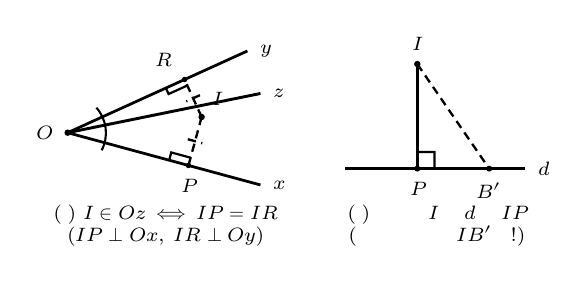
\begin{tikzpicture}[scale=0.83, every node/.style={font=\scriptsize, text=black}]
  % (១) លក្ខណៈសម្គាល់កន្លះបន្ទាត់ពុះមុំ
  \begin{scope}[shift={(0,0)}]
    \coordinate (O) at (-1.45,0);
    \coordinate (X) at (1.50,-0.80);
    \coordinate (Y) at (1.30,1.25);
    \coordinate (M) at (0.60,0.24);
    \coordinate (P) at ($(O)!(M)!(X)$);
    \coordinate (R) at ($(O)!(M)!(Y)$);
    \draw[black, line width=1.0pt] (O) -- (X) node[right=1pt] {$x$};
    \draw[black, line width=1.0pt] (O) -- (Y) node[right=1pt] {$y$};
    \draw[black, line width=1.05pt] (O) -- (1.50,0.60) node[right=1pt] {$z$};
    \draw[black, line width=0.85pt, densely dashed, tk1] (M) -- (P);
    \draw[black, line width=0.85pt, densely dashed, tk1] (M) -- (R);
    \rightbox[0.16]{M}{P}{O}
    \rightbox[0.16]{M}{R}{O}
    \draw[black, line width=0.75pt] ($(O)+(0.52,-0.27)$) arc (-27.5:41.5:0.58);
    \fill[black] (O) circle (1.4pt) node[left=1.5pt] {$O$};
    \fill[black] (M) circle (1.4pt) node[above right=0.5pt] {$I$};
    \fill[black] (P) circle (1.2pt) node[below=1.5pt] {$P$};
    \fill[black] (R) circle (1.2pt) node[above left=1pt] {$R$};
    \node[align=center] at (0.05,-1.42) {(១) $I\in Oz \iff IP = IR$\\($IP\perp Ox,\; IR\perp Oy$)};
  \end{scope}
  % (២) ចំណោលកែងខ្លីជាងអង្កត់ទ្រេត
  \begin{scope}[shift={(4.15,0)}]
    \coordinate (L1) at (-1.35,-0.55);
    \coordinate (L2) at (1.40,-0.55);
    \coordinate (I) at (-0.25,1.05);
    \coordinate (P) at (-0.25,-0.55);
    \coordinate (S) at (0.85,-0.55);
    \draw[black, line width=1.0pt] (L1) -- (L2) node[right=1pt] {$d$};
    \draw[black, line width=1.05pt] (I) -- (P);
    \draw[black, line width=0.85pt, densely dashed] (I) -- (S);
    \rightbox[0.16]{I}{P}{L2}
    \fill[black] (I) circle (1.4pt) node[above=1.5pt] {$I$};
    \fill[black] (P) circle (1.3pt) node[below=1.5pt] {$P$};
    \fill[black] (S) circle (1.3pt) node[below=1.5pt] {$B'$};
    \node[align=center] at (0.05,-1.42) {(២) ចម្ងាយពី $I$ ទៅ $d$ គឺ $IP$\\(មិនមែនអង្កត់ទ្រេត $IB'$ ទេ!)};
  \end{scope}
\end{tikzpicture}}

% ២. E1 Engage: អាងឈូករាងរង្វង់ធំបំផុតប៉ះផ្លូវដើរទាំងបី AB, BC, CA
\newcommand{\figEngageINB}{%
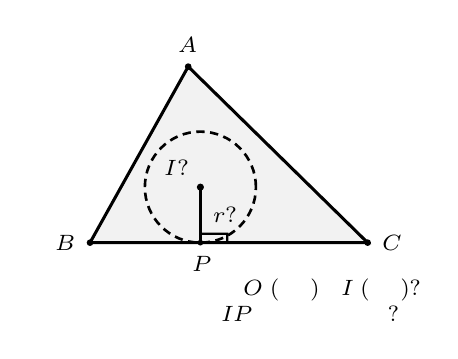
\begin{tikzpicture}[scale=0.86, every node/.style={font=\footnotesize, text=black}]
  \coordinate (B) at (-2.00,-0.80);
  \coordinate (C) at (2.10,-0.80);
  \coordinate (A) at (-0.55,1.80);
  \coordinate (I) at (-0.37,0.02);
  \coordinate (P) at (-0.37,-0.80);
  \fill[gray!10] (A) -- (B) -- (C) -- cycle;
  \draw[black, line width=1.1pt] (A) -- (B) -- (C) -- cycle;
  \draw[black, line width=0.95pt, densely dashed] (I) circle (0.82cm);
  \draw[black, line width=0.85pt] (I) -- (P) node[midway, right=1pt] {$r?$};
  \rightbox[0.16]{I}{P}{C}
  \fill[black] (A) circle (1.4pt) node[above=1.5pt] {$A$};
  \fill[black] (B) circle (1.4pt) node[left=2pt] {$B$};
  \fill[black] (C) circle (1.4pt) node[right=2pt] {$C$};
  \fill[black] (I) circle (1.5pt) node[above left=0.5pt] {$I?$};
  \fill[black] (P) circle (1.2pt) node[below=1.5pt] {$P$};
  \node[align=center] at (0.05,-1.65) {តើផ្ចិតអាងរង្វង់ប៉ះជ្រុងទាំងបីគឺ $O$ (កំពូល) ឬ $I$ (ជ្រុង)?\\តើត្រូវបើកដែកឈានតាមកាំកែង $IP$ ឬតាមចំណុចប្រសព្វទ្រេត?};
\end{tikzpicture}}

% ២ខ. E2 សកម្មភាពទី១៖ ប្រៀបធៀបកាំកែង IP (រង្វង់ប៉ះជ្រុងល្មម) ទល់នឹងអង្កត់ទ្រេត IB' (រង្វង់លៀនចេញក្រៅ)
\newcommand{\figLabINB}{%
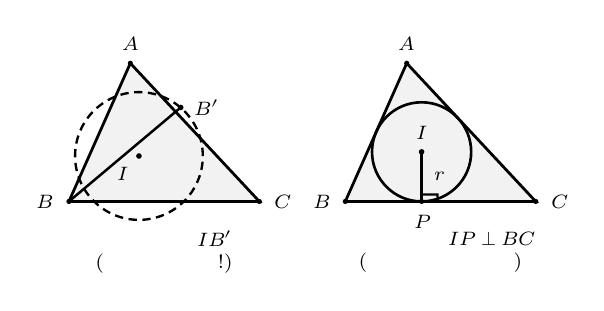
\begin{tikzpicture}[scale=0.78, every node/.style={font=\scriptsize, text=black}]
  % (១) ខុស៖ ឈានដែកឈានតាមអង្កត់ទ្រេត IB' (លៀនចេញក្រៅជ្រុង)
  \begin{scope}[shift={(0,0)}]
    \coordinate (B) at (-1.45,-0.80);
    \coordinate (C) at (1.65,-0.80);
    \coordinate (A) at (-0.45,1.45);
    \coordinate (I) at (-0.31,-0.06);
    \coordinate (Bp) at (0.37,0.73);
    \fill[gray!10] (A) -- (B) -- (C) -- cycle;
    \draw[black, line width=1.0pt] (A) -- (B) -- (C) -- cycle;
    \draw[black, line width=0.85pt, densely dashed] (I) circle (1.04cm);
    \draw[black, line width=0.9pt] (B) -- (Bp);
    \fill[black] (A) circle (1.2pt) node[above=1pt] {$A$};
    \fill[black] (B) circle (1.2pt) node[left=2pt] {$B$};
    \fill[black] (C) circle (1.2pt) node[right=2pt] {$C$};
    \fill[black] (I) circle (1.3pt) node[below left=0.5pt] {$I$};
    \fill[black] (Bp) circle (1.3pt) node[right=1.5pt] {$B'$};
    \node[align=center] at (0.10,-1.62) {ខុស៖ បើកដែកឈានតាម $IB'$\\(រង្វង់លៀនចេញក្រៅជ្រុង!)};
  \end{scope}
  % (២) ត្រូវ៖ ទម្លាក់ចំណោលកែង IP ⊥ BC (ប៉ះជ្រុងទាំងបីល្មម)
  \begin{scope}[shift={(4.50,0)}]
    \coordinate (B) at (-1.45,-0.80);
    \coordinate (C) at (1.65,-0.80);
    \coordinate (A) at (-0.45,1.45);
    \pgfmathsetmacro{\la}{3.10}
    \pgfmathsetmacro{\lb}{veclen(2.10,2.25)}
    \pgfmathsetmacro{\lc}{veclen(1.00,2.25)}
    \pgfmathsetmacro{\per}{\la+\lb+\lc}
    \pgfmathsetmacro{\ix}{(\la*(-0.45)+\lb*(-1.45)+\lc*(1.65))/\per}
    \pgfmathsetmacro{\iy}{(\la*(1.45)+\lb*(-0.80)+\lc*(-0.80))/\per}
    \coordinate (I) at (\ix,\iy);
    \coordinate (P) at (\ix,-0.80);
    \pgfmathsetmacro{\rad}{\iy+0.80}
    \fill[gray!10] (A) -- (B) -- (C) -- cycle;
    \draw[black, line width=1.0pt] (A) -- (B) -- (C) -- cycle;
    \draw[black, line width=0.95pt] (I) circle (\rad cm);
    \draw[black, line width=0.9pt] (I) -- (P) node[midway, right=1pt] {$r$};
    \rightbox[0.14]{I}{P}{C}
    \fill[black] (A) circle (1.2pt) node[above=1pt] {$A$};
    \fill[black] (B) circle (1.2pt) node[left=2pt] {$B$};
    \fill[black] (C) circle (1.2pt) node[right=2pt] {$C$};
    \fill[black] (I) circle (1.3pt) node[above=1pt] {$I$};
    \fill[black] (P) circle (1.2pt) node[below=1.5pt] {$P$};
    \node[align=center] at (0.10,-1.62) {ត្រូវ៖ ទម្លាក់កែង $IP\perp BC$\\(រង្វង់ប៉ះជ្រុងទាំងបីសុក្រឹត)};
  \end{scope}
\end{tikzpicture}}

% ៣. E2/E3 ឧទាហរណ៍ និងទ្រឹស្តីបទកន្លះបន្ទាត់ពុះមុំក្នុង និងរង្វង់ចារឹកក្នុង (ទំ.២១០–២១១)
\newcommand{\figIncenterProof}{%
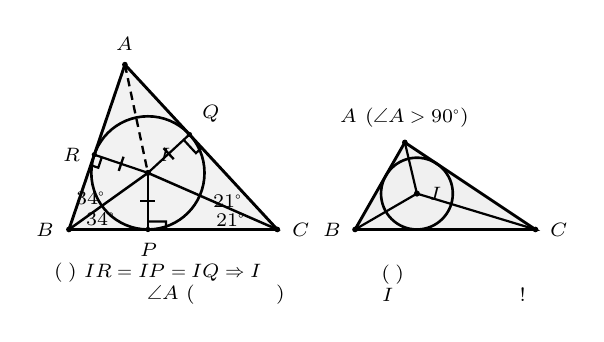
\begin{tikzpicture}[scale=0.79, every node/.style={font=\scriptsize, text=black}]
  % (ក) ឧទាហរណ៍ ទំ.២១០–២១១ (34°, 34° និង 21°, 21°)
  \begin{scope}[shift={(0,0)}]
    \coordinate (B) at (-1.50,-0.95);
    \coordinate (C) at (1.85,-0.95);
    \coordinate (A) at (-0.60,1.70);
    \pgfmathsetmacro{\la}{3.35}
    \pgfmathsetmacro{\lb}{veclen(2.45,2.65)}
    \pgfmathsetmacro{\lc}{veclen(0.90,2.65)}
    \pgfmathsetmacro{\per}{\la+\lb+\lc}
    \pgfmathsetmacro{\ix}{(\la*(-0.60)+\lb*(-1.50)+\lc*(1.85))/\per}
    \pgfmathsetmacro{\iy}{(\la*(1.70)+\lb*(-0.95)+\lc*(-0.95))/\per}
    \coordinate (I) at (\ix,\iy);
    \coordinate (P) at (\ix,-0.95);
    \coordinate (Q) at ($(A)!(I)!(C)$);
    \coordinate (R) at ($(A)!(I)!(B)$);
    \pgfmathsetmacro{\rad}{\iy+0.95}

    \fill[gray!10] (A) -- (B) -- (C) -- cycle;
    \draw[black, line width=1.05pt] (A) -- (B) -- (C) -- cycle;
    \draw[black, line width=0.95pt] (I) circle (\rad cm);
    \draw[black, line width=0.9pt] (B) -- (I) (C) -- (I);
    \draw[black, line width=0.85pt, densely dashed] (A) -- (I);
    \draw[black, line width=0.8pt, tk1] (I) -- (P);
    \draw[black, line width=0.8pt, tk1] (I) -- (Q);
    \draw[black, line width=0.8pt, tk1] (I) -- (R);
    \rightbox[0.14]{I}{P}{C}
    \rightbox[0.14]{I}{Q}{C}
    \rightbox[0.14]{I}{R}{B}
    \fill[black] (A) circle (1.3pt) node[above=1.5pt] {$A$};
    \fill[black] (B) circle (1.3pt) node[left=2pt] {$B$};
    \fill[black] (C) circle (1.3pt) node[right=2pt] {$C$};
    \fill[black] (I) circle (1.4pt) node[above right=0.5pt] {$I$};
    \fill[black] (P) circle (1.2pt) node[below=1.5pt] {$P$};
    \fill[black] (Q) circle (1.2pt) node[above right=1pt] {$Q$};
    \fill[black] (R) circle (1.2pt) node[left=1.5pt] {$R$};
    \node at (-0.98,-0.78) {$34^\circ$};
    \node at (-1.14,-0.44) {$34^\circ$};
    \node at (1.10,-0.80) {$21^\circ$};
    \node at (1.05,-0.50) {$21^\circ$};
    \node[align=center] at (0.15,-1.82) {(ក) $IR=IP=IQ \Rightarrow I$ នៅលើ\\កន្លះបន្ទាត់ពុះ $\ang{A}$ (ផ្ចិតចារឹកក្នុង)};
  \end{scope}

  % (ខ) ប្រៀបធៀប៖ ផ្ចិតចារឹកក្នុង I ស្ថិតនៅក្នុងត្រីកោណជានិច្ច (សូម្បីមុំទាល!)
  \begin{scope}[shift={(4.50,0)}]
    \coordinate (B) at (-1.40,-0.95);
    \coordinate (C) at (1.50,-0.95);
    \coordinate (A) at (-0.60,0.45);
    \pgfmathsetmacro{\la}{2.90}
    \pgfmathsetmacro{\lb}{veclen(2.10,1.40)}
    \pgfmathsetmacro{\lc}{veclen(0.80,1.40)}
    \pgfmathsetmacro{\per}{\la+\lb+\lc}
    \pgfmathsetmacro{\ix}{(\la*(-0.60)+\lb*(-1.40)+\lc*(1.50))/\per}
    \pgfmathsetmacro{\iy}{(\la*(0.45)+\lb*(-0.95)+\lc*(-0.95))/\per}
    \coordinate (I) at (\ix,\iy);
    \pgfmathsetmacro{\rad}{\iy+0.95}
    \fill[gray!12] (A) -- (B) -- (C) -- cycle;
    \draw[black, line width=1.05pt] (A) -- (B) -- (C) -- cycle;
    \draw[black, line width=0.95pt] (I) circle (\rad cm);
    \draw[black, line width=0.8pt] (A) -- (I) (B) -- (I) (C) -- (I);
    \fill[black] (A) circle (1.3pt) node[above=2pt] {$A$ ($\ang{A}>90^\circ$)};
    \fill[black] (B) circle (1.3pt) node[left=2pt] {$B$};
    \fill[black] (C) circle (1.3pt) node[right=2pt] {$C$};
    \fill[black] (I) circle (1.4pt) node[right=1.5pt] {$I$};
    \node[align=center] at (0.05,-1.82) {(ខ) ទោះបីត្រីកោណមុំទាល\\ក៏ $I$ ស្ថិតនៅខាងក្នុងជានិច្ច!};
  \end{scope}
\end{tikzpicture}}

% ៤. E4 លំហាត់គំរូ (ទំ.២១២៖ ∠BIC=120° ⇒ សម័ង្ស) និង ប្រតិបត្តិ (ទំ.២១២៖ ∠A=90° ⇒ ∠BIC=135°)
\newcommand{\figElaborateINB}{%
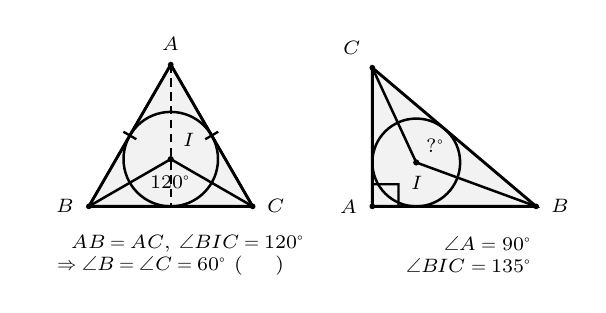
\begin{tikzpicture}[scale=0.80, every node/.style={font=\scriptsize, text=black}]
  % (ក) លំហាត់គំរូ ទំ.២១២
  \begin{scope}[shift={(0,0)}]
    \coordinate (B) at (-1.30,-0.85);
    \coordinate (C) at (1.30,-0.85);
    \coordinate (A) at (0,1.40);
    \coordinate (I) at (0,-0.10);
    \fill[gray!10] (A) -- (B) -- (C) -- cycle;
    \draw[black, line width=1.05pt] (A) -- (B) -- (C) -- cycle;
    \draw[black, line width=0.9pt] (I) circle (0.75cm);
    \draw[black, line width=0.9pt] (B) -- (I) -- (C);
    \draw[black, line width=0.8pt, densely dashed] (A) -- (0,-0.85);
    \draw[black, line width=0.8pt, tk1] (A) -- (B);
    \draw[black, line width=0.8pt, tk1] (A) -- (C);
    \fill[black] (A) circle (1.3pt) node[above=1.5pt] {$A$};
    \fill[black] (B) circle (1.3pt) node[left=2pt] {$B$};
    \fill[black] (C) circle (1.3pt) node[right=2pt] {$C$};
    \fill[black] (I) circle (1.4pt) node[above right=1pt] {$I$};
    \node at (0,-0.46) {$120^\circ$};
    \node[align=center] at (0,-1.62) {គំរូ៖ $AB=AC,\;\ang{BIC}=120^\circ$\\$\Rightarrow \ang{B}=\ang{C}=60^\circ$ (សម័ង្ស)};
  \end{scope}

  % (ខ) ប្រតិបត្តិ ទំ.២១២
  \begin{scope}[shift={(4.35,0)}]
    \coordinate (A) at (-1.15,-0.85);
    \coordinate (B) at (1.45,-0.85);
    \coordinate (C) at (-1.15,1.35);
    \pgfmathsetmacro{\la}{veclen(2.60,2.20)}
    \pgfmathsetmacro{\lb}{2.20}
    \pgfmathsetmacro{\lc}{2.60}
    \pgfmathsetmacro{\rad}{(\lb+\lc-\la)/2}
    \coordinate (I) at (-1.15+\rad,-0.85+\rad);
    \fill[gray!10] (A) -- (B) -- (C) -- cycle;
    \draw[black, line width=1.05pt] (A) -- (B) -- (C) -- cycle;
    \rightbox[0.16]{C}{A}{B}
    \draw[black, line width=0.9pt] (I) circle (\rad cm);
    \draw[black, line width=0.9pt] (B) -- (I) -- (C);
    \fill[black] (A) circle (1.3pt) node[left=2pt] {$A$};
    \fill[black] (B) circle (1.3pt) node[right=2pt] {$B$};
    \fill[black] (C) circle (1.3pt) node[above left=1pt] {$C$};
    \fill[black] (I) circle (1.4pt) node[below=1.5pt] {$I$};
    \node at (-0.15,0.12) {$?^\circ$};
    \node[align=center] at (0.15,-1.62) {ប្រតិបត្តិ៖ $\ang{A}=90^\circ$\\គណនា $\ang{BIC}=135^\circ$};
  \end{scope}
\end{tikzpicture}}

% ៥. E5 លំហាត់ទី៧ (ទំ.២១៣) និងកំណែកិច្ចការផ្ទះទី៦ (ការេ APIQ)
\newcommand{\figEvaluateINB}{%
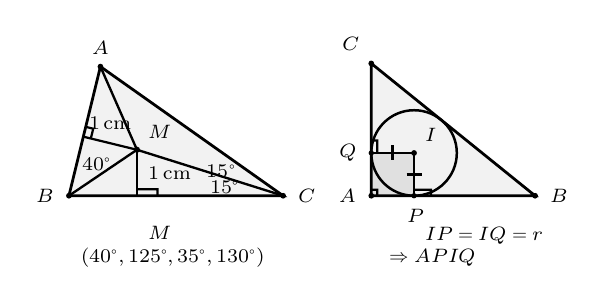
\begin{tikzpicture}[scale=0.80, every node/.style={font=\scriptsize, text=black}]
  % (ក) លំហាត់ទី៧ (ទំ.២១៣)
  \begin{scope}[shift={(0,0)}]
    \coordinate (B) at (-1.50,-0.75);
    \coordinate (C) at (1.90,-0.75);
    \coordinate (A) at (-1.00,1.30);
    \coordinate (M) at (-0.42,-0.02);
    \coordinate (P) at (-0.42,-0.75);
    \coordinate (R) at ($(A)!(M)!(B)$);
    \fill[gray!10] (A) -- (B) -- (C) -- cycle;
    \draw[black, line width=1.0pt] (A) -- (B) -- (C) -- cycle;
    \draw[black, line width=0.85pt] (A) -- (M) (B) -- (M) (C) -- (M);
    \draw[black, line width=0.8pt] (M) -- (P) node[midway, right=0.5pt] {$1\unit{cm}$};
    \draw[black, line width=0.8pt] (M) -- (R) node[midway, above=1pt] {$1\unit{cm}$};
    \rightbox[0.14]{M}{P}{C}
    \rightbox[0.14]{M}{R}{A}
    \fill[black] (A) circle (1.3pt) node[above=1pt] {$A$};
    \fill[black] (B) circle (1.3pt) node[left=2pt] {$B$};
    \fill[black] (C) circle (1.3pt) node[right=2pt] {$C$};
    \fill[black] (M) circle (1.4pt) node[above right=0.5pt] {$M$};
    \node at (-1.06,-0.25) {$40^\circ$};
    \node at (0.98,-0.62) {$15^\circ$};
    \node at (0.92,-0.36) {$15^\circ$};
    \node[align=center] at (0.15,-1.56) {លំហាត់ទី៧៖ $M$ ផ្ចិតចារឹកក្នុង\\($40^\circ, 125^\circ, 35^\circ, 130^\circ$)};
  \end{scope}
  % (ខ) តម្រុយលំហាត់ទី៦៖ ចតុកោណ APIQ ជាការេ
  \begin{scope}[shift={(4.45,0)}]
    \coordinate (A) at (-1.15,-0.75);
    \coordinate (B) at (1.45,-0.75);
    \coordinate (C) at (-1.15,1.35);
    \pgfmathsetmacro{\la}{veclen(2.60,2.10)}
    \pgfmathsetmacro{\rad}{(2.10+2.60-\la)/2}
    \coordinate (I) at (-1.15+\rad,-0.75+\rad);
    \coordinate (P) at (-1.15+\rad,-0.75);
    \coordinate (Q) at (-1.15,-0.75+\rad);
    \fill[gray!10] (A) -- (B) -- (C) -- cycle;
    \fill[gray!24] (A) -- (P) -- (I) -- (Q) -- cycle;
    \draw[black, line width=1.0pt] (A) -- (B) -- (C) -- cycle;
    \draw[black, line width=0.9pt] (I) circle (\rad cm);
    \draw[black, line width=0.85pt, tk1] (I) -- (P);
    \draw[black, line width=0.85pt, tk1] (I) -- (Q);
    \rightbox[0.14]{Q}{A}{P}
    \rightbox[0.14]{I}{P}{B}
    \rightbox[0.14]{I}{Q}{C}
    \fill[black] (A) circle (1.3pt) node[left=2pt] {$A$};
    \fill[black] (B) circle (1.3pt) node[right=2pt] {$B$};
    \fill[black] (C) circle (1.3pt) node[above left=1pt] {$C$};
    \fill[black] (I) circle (1.3pt) node[above right=0.5pt] {$I$};
    \fill[black] (P) circle (1.2pt) node[below=1.5pt] {$P$};
    \fill[black] (Q) circle (1.2pt) node[left=1.5pt] {$Q$};
    \node[align=center] at (0.15,-1.56) {លំហាត់ទី៦៖ $IP=IQ=r$\\$\Rightarrow APIQ$ ជាការេ};
  \end{scope}
\end{tikzpicture}}

% ============================================================================
% ចាប់ផ្ដើមឯកសារ (Document Body)
% ============================================================================
\begin{document}
\fontsize{10pt}{15.2pt}\selectfont

% -------------------- ក្បាលកិច្ចតែងការ (Header) --------------------
\begin{center}
  {\muol\fontsize{11pt}{16pt}\selectfont ព្រះរាជាណាចក្រកម្ពុជា}\\[2pt]
  {\muol\fontsize{10pt}{15pt}\selectfont ជាតិ សាសនា ព្រះមហាក្សត្រ}\\[1pt]
  \khmflourish
\end{center}

\vspace{-26pt}
{\muol\fontsize{9.5pt}{12.8pt}\selectfont
មន្ទីរអប់រំ យុវជន និងកីឡា ខេត្តកំពង់ធំ\\
ការិយាល័យអប់រំ យុវជន និងកីឡា ស្រុកកំពង់ស្វាយ\\
អនុវិទ្យាល័យព្រះក្រសាំង}

\vspace{1pt}
\begin{center}
  {\muol\fontsize{10pt}{14.5pt}\selectfont កិច្ចតែងការបង្រៀន}
\end{center}
\vspace{0pt}

% -------------------- ព័ត៌មានទូទៅ (Metadata) --------------------
{\renewcommand{\arraystretch}{0.98}
\hspace*{4.05cm}%
\begin{tabular}{@{}l l l@{}}
  - \hspace{0.35cm} មុខវិជ្ជា & : & គណិតវិទ្យា ថ្នាក់ទី៨ \\
  - \hspace{0.35cm} ចំណងជើងមេរៀន & : & មេរៀនទី១៦ បន្ទាត់និងអង្កត់ពិសេសជួបគ្នានៅក្នុងត្រីកោណ \\
  - \hspace{0.35cm} ចំណងជើងរង & : & ១៦.៤ លក្ខណៈកន្លះបន្ទាត់ពុះមុំក្នុងនៃត្រីកោណ (ទំព័រ ២១០--២១៣) \\
  - \hspace{0.35cm} រយៈពេល & : & ១ ម៉ោងសិក្សា (៥០ នាទី) \\
  - \hspace{0.35cm} បង្រៀនដោយ & : & ហុក ប៊ុនថែន \\
  - \hspace{0.35cm} កាលបរិច្ឆេទ & : & ថ្ងៃ\makebox[18mm]{\dotfill}\ ទី\makebox[8mm]{\dotfill}\ ខែ\makebox[18mm]{\dotfill}\ ឆ្នាំ២០២៦ \\
\end{tabular}

\vspace{2pt}

% -------------------- I. វត្ថុបំណង --------------------
\textbf{I.} {\muol វត្ថុបំណង}\\[1pt]
\hspace*{0.55cm}%
\begin{tabular}{@{}l l L{14.2cm}@{}}
  \wcirc \hspace{0.25cm} វិជ្ជាសម្បទា & : & សិស្សប្រាប់បានត្រឹមត្រូវពីទ្រឹស្ដីបទប្រសព្វនៃកន្លះបន្ទាត់ពុះមុំក្នុងទាំងបីនៃត្រីកោណ លក្ខណៈស្មើចម្ងាយពីជ្រុងទាំងបី ($IP=IQ=IR$) និងនិយមន័យផ្ចិតរង្វង់ចារឹកក្នុងត្រីកោណ ($I$) ។ \\
  \wcirc \hspace{0.25cm} បំណិនសម្បទា & : & សិស្សសង់ផ្ចិត $I$ និងទម្លាក់ចំណោលកែង $IP$ ដើម្បីគូសរង្វង់ចារឹកក្នុងត្រីកោណ ព្រមទាំងគណនារង្វាស់មុំទាក់ទងនឹងផ្ចិត $I$ បានត្រឹមត្រូវតាមហេតុផលធរណីមាត្រ ។ \\
  \wcirc \hspace{0.25cm} ចរិយាសម្បទា & : & សិស្សមានភាពផ្ចិតផ្ចង់ក្នុងការទម្លាក់ចំណោលកែងរកកាំរង្វង់ចារឹកក្នុង (មិនច្រឡំនឹងអង្កត់ទ្រេត) និងសហការគ្នាពិភាក្សាយ៉ាងសកម្ម ។ \\
\end{tabular}

\vspace{2pt}

% -------------------- II. សម្ភារៈឧបទេស --------------------
\textbf{II.} {\muol សម្ភារៈឧបទេស}\\[1pt]
\hspace*{0.55cm}$\bullet$ \hspace{0.35cm} សៀវភៅសិក្សាគោលគណិតវិទ្យាថ្នាក់ទី៨ (ទំ.២១០--២១៣) សន្លឹកកិច្ចការសិស្ស ស-ខ្មៅ (\en{Worksheet\_INB} ចំនួន ២ ទំព័រ គ្មាន \en{LCD}) ក្ដារខៀន ដីស បន្ទាត់ក្រិត ដែកឈាន អេគែរ និងរ៉ាប់ព័រទ័រ ។

\vspace{2pt}

% -------------------- III. វិធីសាស្រ្តបង្រៀន --------------------
\textbf{III.} {\muol វិធីសាស្រ្តបង្រៀន}\\[1pt]
\hspace*{0.45cm}%
\begin{tabular}{@{}l l L{14.85cm}@{}}
  $\bullet$ \hspace{0.25cm} គោលវិធី & : & សិស្សមជ្ឈមណ្ឌល (សិក្សាតាមរយៈការបំពេញនិងពិសោធន៍លើសន្លឹកកិច្ចការជាគោល គ្មាន \en{LCD}) \\
  $\bullet$ \hspace{0.25cm} យុទ្ធវិធីបង្រៀន & : & ស្ថាបនានិយម គម្រូ \en{5Es} រួមបញ្ចូលការពិសោធប្រៀបធៀបកាំកែងទល់នឹងអង្កត់ទ្រេត (\en{Tangent-Foot Contrast Lab}), សម្រាយបំភ្លឺមានរចនាសម្ព័ន្ធ និងការប្រៀបធៀប $O$ ទល់នឹង $I$ ។ \\
\end{tabular}
}

\vspace{2pt}

% -------------------- IV. ដំណើរការបង្រៀន --------------------
\textbf{IV.} {\muol ដំណើរការបង្រៀន}

\vspace{1pt}

\renewcommand{\arraystretch}{1.15}
\begin{longtable}{|L{5.50cm}|L{7.90cm}|L{4.80cm}|}
\hline
\rowcolor{headgray}
\multicolumn{1}{|c|}{\muol សកម្មភាពគ្រូ} &
\multicolumn{1}{c|}{\muol ខ្លឹមសារមេរៀន} &
\multicolumn{1}{c|}{\muol សកម្មភាពសិស្ស} \\
\hline
\endfirsthead

\hline
\rowcolor{headgray}
\multicolumn{1}{|c|}{\muol សកម្មភាពគ្រូ} &
\multicolumn{1}{c|}{\muol ខ្លឹមសារមេរៀន} &
\multicolumn{1}{c|}{\muol សកម្មភាពសិស្ស} \\
\hline
\endhead

\hline
\endfoot

\hline
\endlastfoot

% ==================== ជំហានទី១ (2 min) ====================
\stepheader{ជំហានទី១ (រដ្ឋបាលថ្នាក់)}
$\bullet$ ពិនិត្យវត្តមាន សណ្ដាប់ធ្នាប់ អនាម័យ និងចែកសន្លឹកកិច្ចការ \en{Worksheet\_INB} ដល់សិស្សគ្រប់គូ \timenote{(2 min)}
&
$\bullet$ រដ្ឋបាលថ្នាក់ និងការត្រៀមបន្ទាត់ក្រិត ដែកឈាន អេគែរ រ៉ាប់ព័រទ័រ និងសន្លឹកកិច្ចការសិស្ស
&
$\circ$ ប្រធានថ្នាក់រាយការណ៍វត្តមាន\par\vspace{2pt}
$\circ$ ទទួលសន្លឹកកិច្ចការ និងត្រៀមឧបករណ៍ \\[3pt]
\hline

% ==================== ជំហានទី២ (9 min: ≤3 + 3 + E1 3) ====================
\stepheader{ជំហានទី២ (កិច្ចការផ្ទះ + រំលឹកមេរៀនចាស់ + ទំនាក់ទំនងមេរៀនថ្មី)}
\timenote{(កំណែកិច្ចការផ្ទះ $\le 3\text{ min}$)}\par\vspace{2pt}
$\bullet$ ហៅសិស្សឡើងបង្ហាញគន្លឹះលំហាត់ទី៩ (ទំ.២១៤) លើក្ដារខៀន
&
\textbf{កំណែកិច្ចការផ្ទះ (ទំ.២១៤ លំហាត់ទី៩ និងទី១០)៖}\par\vspace{1.5pt}
$\bullet$ \textbf{លំហាត់ទី៩៖} ក្នុង $\tri{ABC}$ មាន $AE\perp BC$ និង $BE\perp AC \Rightarrow E$ ជាអរតូសង់នៃ $\tri{ABC} \Rightarrow CE\perp AB \parallel CD \Rightarrow$ \graybox{$\tri{CDE}$ កែងត្រង់ $C$} ។
&
$\circ$ តំណាងឡើងបង្ហាញគន្លឹះលំហាត់ទី៩ \\[3pt]

$\bullet$ ផ្ទៀងផ្ទាត់លំហាត់ទី១០ (ទំ.២១៤) ជាមួយសិស្សទូទាំងថ្នាក់
&
$\bullet$ \textbf{លំហាត់ទី១០៖} បន្ទាត់មធ្យម $IJ\parallel AB\perp AC \Rightarrow IJ\perp AC$; ជាមួយ $AD\perp CI \Rightarrow J$ ជាអរតូសង់នៃ $\tri{ACI} \Rightarrow \graybox{$AI\perp CJ$}$ ។
&
$\circ$ កែផ្ទៀងផ្ទាត់ចម្លើយក្នុងសៀវភៅសរសេរ \\[3pt]

\timenote{(រំលឹកមេរៀនចាស់ 3 min)}\par\vspace{1.5pt}
$\bullet$ សួរទី១៖ «តើចំណុច $I$ ស្ថិតលើកន្លះបន្ទាត់ពុះមុំ $\ang{xOy}$ មានលក្ខណៈស្មើចម្ងាយដូចម្ដេច?»
&
\textbf{រំលឹកបញ្ញត្តិ៖} \ditem \textbf{កន្លះបន្ទាត់ពុះមុំ៖} $I\in Oz \iff$ ស្មើចម្ងាយពីជ្រុងទាំងពីរ ($IP = IR$ ដែល $IP\perp Ox,\; IR\perp Oy$) ។
&
$\circ$ ឆ្លើយ៖ ស្មើចម្ងាយពីជ្រុងទាំងពីរនៃមុំ ($IP=IR$) \\[3pt]

$\bullet$ សួរទី២៖ «តើចម្ងាយពីចំណុច $I$ ទៅបន្ទាត់ $d$ ត្រូវវាស់តាមអង្កត់កែង $IP$ ឬអង្កត់ទ្រេត $IB'$?»
&
\ditem \textbf{ចម្ងាយពីចំណុចទៅបន្ទាត់៖} ត្រូវវាស់តាម \textbf{អង្កត់ចំណោលកែង} ($IP\perp d$) ជានិច្ច (ខ្លីជាងអង្កត់ទ្រេត $IB'$) ។
&
$\circ$ ឆ្លើយ៖ ត្រូវវាស់តាមអង្កត់កែង $IP$ ជានិច្ច \\[3pt]

& \cfig{\figPrereqINB} & \\[3pt]

\fiveE{E1 - Engage} \timenote{(3 min)}\par\vspace{2pt}
$\bullet$ ណែនាំសិស្សអាន \textbf{បេសកកម្មទី១ (E1)} លើសន្លឹកកិច្ចការទំព័រទី១៖\par\vspace{1.5pt}
\hspace*{0.3em}-- «សាលាចង់សង់អាងឈូករាងរង្វង់ធំបំផុតក្នុងសួនត្រីកោណ $\tri{ABC}$ ឱ្យប៉ះផ្លូវដើរទាំងបី $AB, BC, CA$ ស្មើគ្នា ។ តើផ្ចិតអាងគឺ $O$ ឬចំណុចថ្មី $I$? ហើយតើត្រូវបើកដែកឈានតាមកាំកែង $IP$ ឬតាមចំណុចប្រសព្វទ្រេត?»
&
\textbf{មេរៀនទី១៦៖ បន្ទាត់និងអង្កត់ពិសេសជួបគ្នានៅក្នុងត្រីកោណ}\par\vspace{1.5pt}
\textbf{១៦.៤ លក្ខណៈកន្លះបន្ទាត់ពុះមុំនៃត្រីកោណ (កន្លះបន្ទាត់ពុះក្នុង)}\par\vspace{1.5pt}
\ditem \textbf{បញ្ហាបំផុសគំនិត (E1)៖} ការរកផ្ចិតរង្វង់ប៉ះជ្រុងទាំងបីនៃ $\tri{ABC}$ និងអន្ទាក់កាំរង្វង់ (កាំកែង $IP$ ទល់នឹងអង្កត់ទ្រេត) ។
&
$\circ$ អានបេសកកម្មលើសន្លឹកកិច្ចការ\par\vspace{2pt}
$\circ$ គូសធីកទស្សន៍ទាយជាដៃគូ \\[3pt]

& \cfig{\figEngageINB} & \\[3pt]
\hline

% ==================== ជំហានទី៣ (17 min: E2 11 + E3 6) ====================
\stepheader{ជំហានទី៣ (ខ្លឹមសារមេរៀនថ្មី)}
\fiveE{E2 - Explore} \timenote{(11 min — សកម្មភាពទី១ ពិសោធរ៉ាប់ព័រទ័រ អេគែរ និងដែកឈាន៖ 6 min)}\par\vspace{2pt}
$\bullet$ ឱ្យសិស្សធ្វើការជាដៃគូលើ \textbf{ផ្នែកទី១ (ក) ពិសោធន៍ផ្ទៀងផ្ទាត់ផ្ចិត $I$ និងកាំកែង $r$} លើរូបត្រីកោណ $\tri{ABC}$ បោះពុម្ពស្រាប់ (ដែលកន្លះបន្ទាត់ពុះមុំ $\ang{B}$ និង $\ang{C}$ កាត់គ្នាត្រង់ $I$)
&
\textbf{សកម្មភាពរុករកទី១ (ពិសោធលើសន្លឹកកិច្ចការ)៖}\par\vspace{1.5pt}
$1.$ ភ្ជាប់អង្កត់ $AI$ រួចយករ៉ាប់ព័រទ័រវាស់ $\ang{BAI}$ និង $\ang{CAI} \Rightarrow$ ឃើញស្មើគ្នា ($AI$ ជាកន្លះបន្ទាត់ពុះមុំក្នុងនៃ $\ang{A}$)!
&
$\circ$ គូស $AI$ និងវាស់ផ្ទៀងផ្ទាត់ $\ang{BAI}=\ang{CAI}$ \\[3pt]

$\bullet$ ដើរពិនិត្យអន្ទាក់កាំរង្វង់៖ «កុំបើកដែកឈានទៅចំណុច $B'$ ដែល $BI$ កាត់ $AC$! ចូរយកអេគែរទម្លាក់ចំណោលកែង $IP\perp BC,\; IQ\perp AC,\; IR\perp AB$ រួចវាស់ប្រៀបធៀប!»
&
$2.$ \textbf{ពិសោធអន្ទាក់កាំរង្វង់៖} វាស់ឃើញ $IP = IQ = IR = r$ (ខ្លីជាង $IB'$); ពេលឈានដែកឈានកាំ $r=IP$ រង្វង់ប៉ះជ្រុងទាំងបីត្រង់ $P, Q, R$ យ៉ាងសុក្រឹត!
&
$\circ$ ប្រើអេគែរទម្លាក់កែង $IP, IQ, IR$ វាស់ប្រៀបធៀប និងគូសរង្វង់ចារឹកក្នុងដោយដែកឈាន \\[3pt]

& \cfig{\figLabINB} & \\[3pt]

\timenote{(E2 សកម្មភាពទី២៖ សម្រាយបំភ្លឺឧទាហរណ៍ ទំ.២១០--២១១ — 5 min)}\par\vspace{2pt}
$\bullet$ ដឹកនាំសិស្សបំពេញ \textbf{ផ្នែកទី១ (ខ) ឧទាហរណ៍ (ទំ.២១០--២១១)}៖ «បើ $\ang{ABI}=\ang{CBI}=34^\circ$ និង $\ang{BCI}=\ang{ACI}=21^\circ$ តើ $BI$ និង $CI$ ជាអ្វី?»
&
\textbf{ឧទាហរណ៍ (ទំ.២១០--២១១)៖}\par\vspace{1.5pt}
$\bullet$ \textbf{ក.} ដោយ $\ang{ABI}=\ang{CBI}=34^\circ$ និង $\ang{BCI}=\ang{ACI}=21^\circ$ នោះ $BI$ និង $CI$ ជា \textbf{កន្លះបន្ទាត់ពុះមុំក្នុង} នៃ $\ang{B}$ និង $\ang{C}$ ក្នុង $\tri{ABC}$ ។
&
$\circ$ បំពេញចម្លើយ (ក) លើសន្លឹកកិច្ចការ \\[3pt]

$\bullet$ សួរបន្ត៖ «ហេតុអ្វី $IR=IP$ និង $IP=IQ$? តើសមភាព $IR=IQ$ បញ្ជាក់អ្វីចំពោះកន្លះបន្ទាត់ពុះមុំ $\ang{A}$ និងរង្វង់ផ្ចិត $I$?»
&
$\bullet$ \textbf{ខ.} $I$ នៅលើកន្លះបន្ទាត់ពុះ $\ang{B} \Rightarrow IR=IP$; $I$ នៅលើកន្លះបន្ទាត់ពុះ $\ang{C} \Rightarrow IP=IQ \Rightarrow \mathbf{IR=IQ}$ ។\par\vspace{1.5pt}
$\bullet$ ដោយ $I$ នៅក្នុង $\tri{ABC}$ និង $IR=IQ \Rightarrow I$ ឋិតលើកន្លះបន្ទាត់ពុះក្នុងនៃ $\ang{A}$ ។ ដោយ $IP=IQ=IR$ នោះ $P, Q, R$ ស្ថិតលើរង្វង់ផ្ចិត $I$ តែមួយប៉ះជ្រុងទាំងបី ហៅថា \graybox{រង្វង់ចារឹកក្នុងត្រីកោណ $ABC$} ។
&
$\circ$ បំពេញសមភាព $IR=IP=IQ$ និងសន្និដ្ឋានពីប្រសព្វត្រង់ $I$ \\[3pt]

& \cfig{\figIncenterProof} & \\[3pt]

\fiveE{E3 - Explain} \timenote{(6 min)}\par\vspace{2pt}
$\bullet$ ហៅតំណាងគូសង្ខេប រួចគ្រូសរសេរ \textbf{ទ្រឹស្ដីបទ (ទំ.២១១)} លើក្ដារខៀន ឱ្យសិស្សបំពេញ \textbf{ផ្នែកទី២}
&
\textbf{ទ្រឹស្តីបទ (ទំ.២១១)៖}\par\vspace{1.5pt}
កន្លះបន្ទាត់ពុះមុំក្នុងទាំងបីនៃត្រីកោណមួយប្រសព្វគ្នាត្រង់ចំណុចតែមួយដែលឋិតនៅស្មើចម្ងាយពីជ្រុងទាំងបីនៃត្រីកោណនោះ ។ ចំណុចនេះជា \textbf{ផ្ចិតរង្វង់ចារឹកក្នុងត្រីកោណ} ($I$) ។
&
$\circ$ តំណាងគូឡើងបង្ហាញការសន្និដ្ឋាន\par\vspace{2pt}
$\circ$ បំពេញប្រអប់ទ្រឹស្ដីបទលើសន្លឹកកិច្ចការ \\[3pt]

$\bullet$ សួរប្រៀបធៀបលើក្ដារខៀនដើម្បីកុំឱ្យសិស្សច្រឡំ $O$ និង $I$៖ «តើផ្ចិតរង្វង់ចារឹកក្រៅ $O$ និងផ្ចិតរង្វង់ចារឹកក្នុង $I$ ខុសគ្នាត្រង់ណាខ្លះ?»
&
\textbf{តារាងប្រៀបធៀបកុំឱ្យច្រឡំរវាង $O$ និង $I$៖}\par\vspace{2pt}
{\renewcommand{\arraystretch}{1.12}\footnotesize
\begin{tabular}{|L{1.80cm}|L{2.58cm}|L{2.62cm}|}
\hline
\cellcolor{headgray}\textbf{លក្ខណៈ} & \cellcolor{headgray}\textbf{ផ្ចិតចារឹកក្រៅ $O$ (១៦.២)} & \cellcolor{headgray}\textbf{ផ្ចិតចារឹកក្នុង $I$ (១៦.៤)} \\[2pt]
\hline
បន្ទាត់ប្រសព្វ & មេដ្យាទ័រទាំង ៣ & កន្លះបន្ទាត់ពុះមុំក្នុង ៣ \\
\hline
ស្មើចម្ងាយពី & កំពូលទាំង ៣ ($OA=OB=OC$) & ជ្រុងទាំង ៣ ($IP=IQ=IR$) \\
\hline
ទីតាំងក្នុង $\tri{}$ & ក្នុង / កណ្ដាលអ៊ីប៉ូ. / ក្រៅ & \textbf{នៅខាងក្នុងជានិច្ច!} \\
\hline
\end{tabular}}
&
$\circ$ ប្រៀបធៀបភាពខុសគ្នារវាង $O$ (កំពូល) និង $I$ (ជ្រុង) \\[3pt]

$\bullet$ ណែនាំធនាគារហេតុផល \cnum{1}--\cnum{5} សម្រាប់ដោះស្រាយលំហាត់មុំ និងរង្វង់ចារឹកក្នុង
&
\textbf{ធនាគារហេតុផល (\en{Warrant Bank})៖}\par\vspace{1.5pt}
\cnum{1} និយមន័យកន្លះបន្ទាត់ពុះមុំ ($\ang{IBC}=\frac{\ang{B}}{2}$) \;\textbar\; \cnum{2} ស្មើចម្ងាយពីជ្រុង ($IP=IQ=IR$)\par\vspace{1.5pt}
\cnum{3} ប្រសព្វកន្លះបន្ទាត់ពុះមុំ ២ $\Rightarrow$ ទី ៣ កាត់តាម $I$\par\vspace{1.5pt}
\cnum{4} ផលបូកមុំក្នុងត្រីកោណ ($180^\circ$) \;\textbar\; \cnum{5} បន្ទាត់ប៉ះរង្វង់កែងនឹងកាំ ($IP\perp BC$)
&
$\circ$ ផ្ទៀងផ្ទាត់ធនាគារហេតុផល \cnum{1}--\cnum{5} \\[3pt]
\hline

% ==================== ជំហានទី៤ (20 min: E4 10 + E5 10) ====================
\stepheader{ជំហានទី៤ (ពង្រីកចំណេះដឹង និងវាយតម្លៃ)}
\fiveE{E4 - Elaborate} \timenote{(10 min — លំហាត់គំរូ ទំ.២១២៖ 5 min)}\par\vspace{2pt}
$\bullet$ ដឹកនាំសិស្សអានប្រធាន \textbf{ផ្នែកទី៣ (ក) លំហាត់គំរូ (ទំ.២១២)} លើសន្លឹកកិច្ចការទំព័រទី២៖ «បើ $\tri{ABC}$ សមបាតកំពូល $A$ ហើយ $I$ ជាផ្ចិតរង្វង់ចារឹកក្នុង តើ $\ang{IBC}$ និង $\ang{BCI}$ មានទំនាក់ទំនងអ្វី?»
&
\textbf{លំហាត់គំរូ (ទំ.២១២)៖} $\tri{ABC}$ សមបាតកំពូល $A$, $I$ ជាផ្ចិតរង្វង់ចារឹកក្នុង និង $\ang{BIC}=120^\circ$ ។ ស្រាយបំភ្លឺថា $\tri{ABC}$ ជាត្រីកោណសម័ង្ស៖\par\vspace{1.5pt}
-- ដោយ $I$ ជាផ្ចិតចារឹកក្នុង និង $\ang{B}=\ang{C}$ នោះ $\ang{IBC}=\ang{BCI}=\frac{\ang{B}}{2}=\frac{\ang{C}}{2}$ (\cnum{1}) ។
&
$\circ$ អានប្រធាន និងបំពេញទំនាក់ទំនង $\ang{IBC}=\ang{BCI}=\frac{\ang{B}}{2}$ \\[3pt]

$\bullet$ សួរបញ្ចប់៖ «ក្នុង $\tri{BIC}$ បើ $\ang{BIC}=120^\circ$ តើ $\ang{IBC}$ ស្មើប៉ុន្មានដឺក្រេ? ទាញរក $\ang{B}$ និង $\ang{C}$!»
&
-- ក្នុង $\tri{BIC}$ (\cnum{4})៖ $\ang{IBC}+\ang{BCI}=180^\circ-120^\circ=60^\circ \Rightarrow 2\ang{IBC}=60^\circ \Rightarrow \ang{IBC}=30^\circ$ ។\par\vspace{1.5pt}
-- គេបាន $\frac{\ang{B}}{2}=30^\circ \Rightarrow \ang{B}=\ang{C}=60^\circ$ ។ ត្រីកោណសមបាតមានមុំបាត $60^\circ \Rightarrow$ \graybox{$\tri{ABC}$ ជាត្រីកោណសម័ង្ស}!
&
$\circ$ គណនា $\ang{IBC}=30^\circ \Rightarrow \ang{B}=\ang{C}=60^\circ$ (ត្រីកោណសម័ង្ស) \\[3pt]

\timenote{(E4 ប្រតិបត្តិ៖ ទំ.២១២ — 5 min)}\par\vspace{2pt}
$\bullet$ ដឹកនាំសិស្សដោះស្រាយ \textbf{ផ្នែកទី៣ (ខ) ប្រតិបត្តិ (ទំ.២១២)}៖ «បើ $\tri{ABC}$ កែងត្រង់ $A$ តើផលបូក $\ang{B}+\ang{C}$ ស្មើប៉ុន្មាន? ចុះ $\ang{IBC}+\ang{ICB}$?»
&
\textbf{ប្រតិបត្តិ (ទំ.២១២)៖} $\tri{ABC}$ កែងត្រង់កំពូល $A$ ($\ang{A}=90^\circ$) និង $I$ ជាផ្ចិតរង្វង់ចារឹកក្នុង ។ គណនា $\ang{BIC}$ ៖\par\vspace{1.5pt}
$1.$ ក្នុង $\tri{ABC}$ កែងត្រង់ $A$៖ $\ang{B}+\ang{C}=90^\circ \Rightarrow \ang{IBC}+\ang{ICB}=\frac{\ang{B}+\ang{C}}{2}=\frac{90^\circ}{2}=45^\circ$ (\cnum{1}) ។
&
$\circ$ គណនាផលបូកកន្លះមុំ $\ang{IBC}+\ang{ICB}=45^\circ$ \\[3pt]

$\bullet$ សួរបញ្ចប់ និងឆ្លុះបញ្ចាំង (\en{Looking-Back})៖ «តើ $\ang{BIC}$ ស្មើប៉ុន្មានដឺក្រេ? ជាទូទៅ តើ $\ang{BIC}$ ស្មើប៉ុន្មានជាអនុគមន៍នៃ $\ang{A}$?»
&
$2.$ ក្នុង $\tri{BIC}$៖ $\ang{BIC}=180^\circ-(\ang{IBC}+\ang{ICB})=180^\circ-45^\circ=\graybox{$135^\circ$}$ ។\par\vspace{1.5pt}
$\bullet$ \textbf{សង្កេតទូទៅ៖} គ្រប់ត្រីកោណ $\tri{ABC}$ គេមាន $\ang{BIC}=90^\circ+\frac{\ang{A}}{2}$!
&
$\circ$ បំពេញ $\ang{BIC}=135^\circ$ និងផ្ទៀងផ្ទាត់រូបមន្តទូទៅ $90^\circ+\frac{\ang{A}}{2}$ \\[3pt]

& \cfig{\figElaborateINB} & \\[3pt]

\fiveE{E5 - Evaluate} \timenote{(10 min — លំហាត់ទី៧ ទំ.២១៣៖ 6 min)}\par\vspace{2pt}
$\bullet$ ឱ្យសិស្សធ្វើ \textbf{ផ្នែកទី៤ (ក) លំហាត់ទី៧ (ទំ.២១៣)} ដោយឯករាជ្យលើសន្លឹកកិច្ចការ (សង្កេតអង្កត់កែង $1\unit{cm}$ ស្មើគ្នាពី $M$ ទៅ $AB$ និង $BC$)
&
\textbf{រង្វាយតម្លៃទី១ — លំហាត់ទី៧ (ទំ.២១៣)៖}\par\vspace{1.5pt}
$\bullet$ ដោយ $M$ ស្មើចម្ងាយ ($1\unit{cm}=1\unit{cm}$) ពី $BA$ និង $BC \Rightarrow BM$ ជាកន្លះបន្ទាត់ពុះ $\ang{B} \Rightarrow \mathbf{\ang{MBC}}=\ang{ABM}=\mathbf{40^\circ}$ ($\ang{B}=80^\circ$) ។\par\vspace{1.5pt}
$\bullet$ ក្នុង $\tri{MBC}$ ($\ang{MCB}=15^\circ$)៖ $\mathbf{\ang{BMC}}=180^\circ-(40^\circ+15^\circ)=\mathbf{125^\circ}$ ។
&
$\circ$ សម្គាល់ហេតុផល \cnum{2} ទាញបាន $\ang{MBC}=40^\circ$ និង $\ang{BMC}=125^\circ$ \\[3pt]

$\bullet$ ហៅសិស្សបង្ហាញការគណនា $\ang{CAM}$ និង $\ang{AMC}$ ដើម្បីបំពេញតារាងទាំង ៤ ប្រអប់
&
$\bullet$ ដោយ $BM$ និង $CM$ ($15^\circ=15^\circ \Rightarrow \ang{C}=30^\circ$) ប្រសព្វត្រង់ $M \Rightarrow M$ ជាផ្ចិតចារឹកក្នុង (\cnum{3}) ហើយ $\ang{A}=180^\circ-(80^\circ+30^\circ)=70^\circ \Rightarrow \mathbf{\ang{CAM}}=\frac{70^\circ}{2}=\mathbf{35^\circ}$ ។\par\vspace{1.5pt}
$\bullet$ ក្នុង $\tri{AMC}$៖ $\mathbf{\ang{AMC}}=180^\circ-(35^\circ+15^\circ)=\mathbf{130^\circ}$ ។
&
$\circ$ បំពេញតារាងពេញលេញ៖ $40^\circ,\; 125^\circ,\; 35^\circ,\; 130^\circ$ \\[3pt]

& \cfig{\figEvaluateINB} & \\[3pt]

\timenote{(E5 បិទបេសកកម្ម E1 និង \en{Exit Check} — 4 min)}\par\vspace{2pt}
$\bullet$ សួរបិទបេសកកម្មអាងឈូករាងរង្វង់ E1 ពីដើមម៉ោង និងឱ្យសិស្សគូសវង់ \textbf{\en{Exit Check} (ផ្នែកទី៤ ខ)}
&
\textbf{រង្វាយតម្លៃទី២ — បិទ E1 និង \en{Exit Check}៖}\par\vspace{1.5pt}
$\bullet$ \textbf{ចម្លើយ E1៖} ត្រូវរកផ្ចិត $I$ (ប្រសព្វកន្លះបន្ទាត់ពុះមុំក្នុង) និងបើកដែកឈានតាមកាំកែង $IP\perp BC$ ។\par\vspace{1.5pt}
$\bullet$ \textbf{\en{Exit Check}៖} សំណួរទី១ $\to$ \textbf{ខ} ($IP=IQ=IR$); សំណួរទី២ $\to$ \textbf{ក} (អង្កត់កែង $IP$); សំណួរទី៣ $\to$ \textbf{ក} (នៅខាងក្នុងជានិច្ច) ។
&
$\circ$ ផ្ទៀងផ្ទាត់ការទស្សន៍ទាយ E1\par\vspace{2pt}
$\circ$ គូសវង់ \en{Exit Check} និងលើកម្រាមដៃបង្ហាញ \\[3pt]
\hline

% ==================== ជំហានទី៥ (≤2 min) ====================
\stepheader{ជំហានទី៥ (កិច្ចការផ្ទះ + បណ្ដាំផ្ញើ)}
\timenote{(ចំណាយពេល $\le 2\text{ min}$)}\par\vspace{2pt}
$\bullet$ ដាក់កិច្ចការផ្ទះពីសៀវភៅសិក្សាគោល (ទំ.២១៣--២១៤)
&
\centerline{\muol កិច្ចការផ្ទះ \enbf{(}ទំ\enbf{.}២១៣\enbf{--}២១៤ លំហាត់ទី៦ និងទី១២\enbf{)}}\par\vspace{2pt}
$1.$ \textbf{លំហាត់ទី៦ (ទំ.២១៣)៖} $\tri{ABC}$ កែងត្រង់ $A$ ។ រង្វង់ចារឹកក្នុងត្រីកោណនេះប៉ះជ្រុងត្រង់ $P, Q, R$ ($I$ ជាផ្ចិត) ។ ប្រាប់ប្រភេទនៃចតុកោណ $APIQ$ \textit{(គន្លឹះ៖ ពិនិត្យមុំកែង ៣ និងជ្រុងជាប់គ្នា $IP=IQ=r$)} ។
&
$\circ$ កត់ត្រាលំហាត់ទី៦ និងគន្លឹះដោះស្រាយ \\[3pt]

$\bullet$ ណែនាំលំហាត់ទី១២ (ផ្នែករំលឹក) និងផ្ដាំផ្ញើអានមេរៀនបញ្ចប់នៃមេរៀនទី១៦
&
$2.$ \textbf{លំហាត់ទី១២ (ទំ.២១៤)៖} ក្នុង $\tri{ABC}$ កន្លះបន្ទាត់ពុះមុំ $B$ និង $C$ ប្រសព្វត្រង់ $I$; ក្នុង $\tri{ADE}$ កន្លះបន្ទាត់ពុះមុំ $D$ និង $E$ ប្រសព្វត្រង់ $J$ ។ បង្ហាញថា $A, I, J$ រត់ត្រង់ជួរគ្នា ។\par\vspace{1.5pt}
$3.$ \textbf{អានជាមុន៖} ចំណុច \textbf{កន្លះបន្ទាត់ពុះក្រៅនិងកន្លះបន្ទាត់ពុះក្នុង} (ទំ.២១១--២១២) និងត្រៀមដែកឈាន អេគែរ បន្ទាត់ក្រិត ។
&
$\circ$ កត់ត្រាលំហាត់ទី១២ និងចំណុចអានជាមុន\par\vspace{2pt}
$\circ$ ជម្រាបលាលោកគ្រូ \\[3pt]
\end{longtable}

% -------------------- កាលបរិច្ឆេទ និងហត្ថលេខា --------------------
\vspace{10pt}
\hfill
\begin{minipage}{9.8cm}
  {\centering
    ថ្ងៃ\makebox[16mm]{\dotfill}\ ខែ\makebox[18mm]{\dotfill}\ ឆ្នាំមមី អដ្ឋស័ក ពុទ្ធសករាជ ២៥៧០\\[2pt]
    កំពង់ស្វាយ, ថ្ងៃទី\makebox[10mm]{\dotfill}\ ខែ\makebox[18mm]{\dotfill}\ ឆ្នាំ២០២៦\\[3pt]
    {\muol គ្រូបង្រៀន}\par}
  \vspace{32pt}
  \hfill{\muol ហុក ប៊ុនថែន}\hspace*{1.4cm}
\end{minipage}

\end{document}
